\svnkwsave{$RepoFile: siminos/spatiotemp/chapter/homology.tex $}
\svnidlong {$HeadURL: svn://zero.physics.gatech.edu/siminos/spatiotemp/chapter/homology.tex $}
{$LastChangedDate: 2020-05-22 16:09:57 -0400 (Fri, 22 May 2020) $}
{$LastChangedRevision: 6836 $} {$LastChangedBy: predrag $}
\svnid{$Id: homology.tex 6836 2019-04-18 03:47:17Z predrag $}

\chapter{Persistent homology}
\label{chap:homology}
% Predrag                                           29 Oct 2018
%      extracted from blogMNG.tex

\begin{description}

\NBBpost{2018-07-05}{
A possible method to systematically classifying the
patterns could be the
\href{https://en.wikipedia.org/wiki/Persistent_homology}{persistent homology}.
Matt, If you could generate a large spatiotemporal plot along and a
corresponding peak-detected version, then I can take them to
\href{http://pub.ist.ac.at/~edels/}{Herbert Edelsbrunner} and ask for his
advice on how to go about extracting a finite library of patterns.
}

\MNGpost{2018-09-11}{
{\bf [Persistent homology]}
Spent the morning searching through literature on
persistent homology in conjunction with pattern detection,
partial differential equations. I have about ten papers that
I need to add them to the bib but I need to skim them to
pick out the good ones first.

Set-up a meeting for tomorrow at 3:00 pm.
with Brett Tregoning from the Schatz'
group to discuss their \refref{KLTSPSM16}
\textit{Analysis of Kolmogorov Flow and Rayleigh-B\'enard Convection using Persistent
Homology} and to get a general introduction on the
subject.
}

\MNGpost{2018-09-12}{
Happy Birthday to me. Now back to work.

\begin{description}
\item[Konstantin Mischaikow Seminar on Persistent Homology]
\HREF{https://youtu.be/IV50VdIuhkA}{Youtube}
The audio cuts in and out so be warned its annoying to listen to.

\item[Talked to Brett Tregoning]
Went through the idea of persistent homology. He recommends (as do I)
watching the videos to get an idea on persistent diagrams in the
supplementary materials at
    \PC{2018-09-25}{``at'' what? \refRef{KLTSPSM16}?}

\item[PHAT]
I can't believe that I have to say this again but I spent an incredibly frustrating amount of time trying to
install a different package to be able to run persistent
homology code in Python, as opposed to writing my own code.

Little did I know that the developers have not updated the description of their package on their webpage since
circa 2013, but it's a fools errand to attempt to install it on a Windows machine. It's almost comical
because their installation instructions literally include only one command line, \texttt{pip install phat}. Only after five hours did I realize that they
did not update the dependencies required for the Windows version, but perhaps I should have known what it meant for the ``Python Bindings'' to only work on linux and MacOS.

Maybe I'm stupid for not exclusively working in Linux land but the documentation for packages written without
an installer is really terrible.

Going to attempt to install a different package named Perseus next, or just only run phat from Light terminal.

\end{description}
}

\MNGpost{2018-09-14}{
\begin{description}
\item[Persistent Homology]
Testing implementations on Linux running
Ubuntu to see what persistent homology
code will be easiest to implement. Out of Rachel Levanger's
\HREF{https://github.com/rachellevanger/tda-persistence-explorer}(tda-persistent-homology) package, Perseus \HREF{http://people.maths.ox.ac.uk/nanda/perseus/index.html}(perseus)
and the barebones PHAT package \HREF{https://pypi.org/project/phat/}(PHAT) (the framework that Rachel Levanger's
code is built upon.

I think the easiest is going to be Rachel Levanger's code because its setup to take a folder of
greyscale images and create the corresponding persistence diagrams. Therefore it should be
somewhat easy to reproduce figures for families of solutions and pass them to these Python functions.
The downside for me is that my main machines are Windows based and this is only active on Linux, so I
will have to see if there are any permission issues in regards to the installation process; I think I should
be fine but I had to find work arounds for channelflow 2.0.

The other two might are not nearly as expedient but if something comes out of Rachel Levanger's codes then
it might be worthwhile to learn the PHAT framework and write my own codes.
\end{description}
}

\begin{figure}[ht]
\begin{minipage}[height=.32\textheight]{.45\textwidth}
\centering \small{\texttt{(a)}}
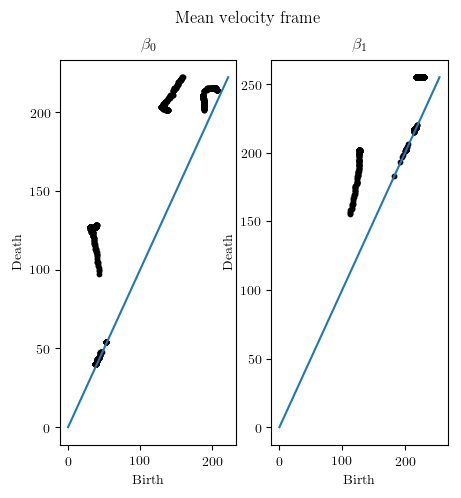
\includegraphics[width=\textwidth,height=.32\textheight]{MNGmvfPE}
\end{minipage}
\begin{minipage}[height=.32\textheight]{.45\textwidth}
\centering \small{\texttt{(b)}}
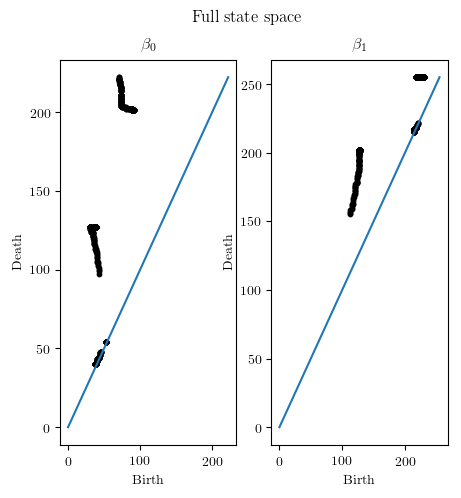
\includegraphics[width=\textwidth,height=.32\textheight]{MNGfullsspPE}
\end{minipage}
\caption{ \label{fig:MNGtestPEdiagrams}
(a) Persistence diagrams for hook family in mean velocity frame (doubly-periodic representation)
(b) Persistence diagrams for hook family of solutions in full state-space. Evidence that code
doesn't support periodic boundary conditions or else these two plots would be the same.
}
\end{figure}

\MNGpost{09-18-2018}{
\begin{description}
\item[Persistent Homology]
Went through testing of Rachel Levanger's %\texttt{Persistence explorer}
Python module. While I can get the persistent homology code to run it
seems that in the documentation that periodic boundary conditions
haven't been implemented yet; although this seemingly contradicts the
data that I saw for two dimensional Kolmogorov flow in the supplemental
materials for the \refref{KLTSPSM16}.

The whole idea is that it is supposed to be picking out
topological information, specifically, for a scalar field $u(x,t)$ and its
image under a homeomorphism $g \circ u(x,t)$ should have the same ``Persistence
Diagrams'' but \reffig{fig:MNGtestPEdiagrams} shows otherwise. Attempting this with relative periodic \twot\ solutions in the
mean-velocity frame and full \statesp\ leads to two different persistence
diagrams, thereby somehow encoding the quantitative difference of the doubly
periodic nature in the mean velocity frame.

I am going to attempt to establish contact with the author of the code
to see if there is any way to adapt my images to be able to utilize
the code properly.

\item[Explanation of persistence diagrams]
The general concept regard persistence diagrams is fairly straightforward; its only
the details of the algorithmic implementation when it gets tricky.

If we imagine a two
dimensional scalar field $u(x,t)$ as a topographical height map, and then we imagine scanning through
the landscape with a constant valued plane $f(\theta)$ (which is easiest to visualize as the ``sea-level'')
that defines sublevel sets $\{u(x,t) : u(x,t) \leq f(\theta)\}$, then we can count the number
of topologically distinct components, labeled by the $n^{\text{th}}$ \emph{Betti number}, $\beta_n$.
The first three Betti numbers can be described by the following: $\beta_0$ counts the number of connected components,
$\beta_1$ counts the number of one-dimensional holes, and $\beta_2$ counts number of voids or ``cavities''
(not applicable with two dimensional scalar fields). In this case, these components are defined with respect to the
sub-level sets or ``sea-level''. Connected regions above sea-level define
    \PC{2018-09-25}{``define'' what?}

To get an intuition for these quantities it is probably easiest to watch the
supplementary videos
\HREF{https://www.sciencedirect.com/science/article/pii/S0167278916000270}
{(click here)} for Schatz group's persistent homology paper\rf{KLTSPSM16}.

What one sees in \reffig{fig:MNGtestPEdiagrams} are the compilation of persistence diagrams for the family of solutions
of the \KSe\ associated with the ``hook'' or ``defect'' pattern, in the
(a) mean velocity frame and in the
(b) full \statesp.
Because these are continuous families of solutions, there should be continuity in the space of persistence diagrams.

The troubling evidence shown in \reffig{fig:MNGtestPEdiagrams} is that the data displayed is supposed to be invariant under
homeomorphisms. I believe that this Python package is not taking the periodic boundary conditions into
account and therefore cannot be fully utilized at this point.

\MNGedit{Confirmed by Rachel Levanger, does not support periodic boundary conditions}
\end{description}
}

\MNGpost{2018-09-24}{
\begin{description}
\item[Persistent Homology]
Schatz' group forgot to bring it up in their weekly
meeting but they believe that Miroslav Kram\'ar  perhaps produced a persistent homology calculation with
the doubly periodic 2-D Kolmogorov flow numerical data (as opposed to experimental data).

Michael Schatz made a comment about a small difference between persistent homology
of two dimensional scalar fields with and without periodic boundary conditions. Coding-wise there
are distinctions because one needs to make sure to not overcount the connected sub-level sets or else
the persistence diagram will not be mathematically consistent between different images, \ie, the technique
is useless if not written specifically to take periodic boundary conditions into consideration. I believe the point
he was trying to make is that because we are working with a topological torus
there is the emergence of a single birth-death event on the $\beta_2$ (Betti number equals two) diagram,
which counts the number of ``cavities'' (think of iso-vorticity surfaces) of the torus.
I believe for him that this is just a trivial piece of information
due to the topology of tori; there is an ``inside'' to the two dimensional
surface, therefore a $\beta_2$ birth-death event occurs.

I reached out to Dr. Kram\'ar, asked him that he share his algorithms with me.

He replied and pointed me towards a library named \texttt{GUDHI} (it's almost like its saying ``Hi Gudorf!'' so maybe its a sign) that uses cubical complexes (fancy words to say that it tracks the level sets
where scalar field $u(x,t) < \theta$) on a lattice to produce the persistence diagrams. I'm hoping to get this
up and running soon.
\end{description}
}


\MNGpost{2018-09-25}{
%There was a huge dump of messages when trying to install GUDHI on light; I can't
%run ``make install'' to install the library so I will need to get Predrag's credentials
%one more time.

All of the documentation is laid out so much better than some other libraries that I've
recently dealt with and it seems that its a relatively widely used library, see
\HREF{http://gudhi.gforge.inria.fr/}{(GUDHI code website)}.

While the only thing I need to do is ``make install'' and then test with ``make test,''
the input file needs to be of a very specific format and the output seems to be of a very
specific format so it looks like I will be writing some python scripts to be able to use
the library. First, I need to use the same algorithm (either custom or built-in) that takes
a greyscale bitmap image and converts it to numbers $n \in [0,255]$ to represent the \twot\
in the correct way.

The input file must list the following, the first line lists the dimension $d=2$ of the array
to be input. Next the negative of the number of rows and columns \textbf{negative for periodic boundary conditions}
$-N$ and $-M$ are listed on successive lines.

Lastly the bitmap data of the scalar field (in my case a matrix) is flattened into a vector, starting at the
bottom left of the field.

So, for example, the following ``data''
\beq
U = \begin{bmatrix}
    7 & 8 & 9 \\
    4 & 5 & 6 \\
    1 & 2 & 3 \\
    \end{bmatrix}
\eeq
would be represented by a text file written exactly as such,

2 (number of dimensions) \\
-3 (number of rows, periodic boundary conditions imply negative) \\
-3 (number of rows, periodic boundary conditions imply negative) \\
1 \\
2 \\
3 \\
4 \\
5 \\
6 \\
7 \\
8 \\
9 \\

The output is a text file containing the lists of births and deaths of different
Betti number components. I do not believe that this has plotting functionality
so I'll take the output and run it through a python script that processes the data
and plots the persistence diagrams of the \twot. I kind of wished that
    \PC{2018-09-26}{`wished that'' what?}
    \PC{2018-09-26}{ Is \reffig{fig:MNG_hookPDdiagram_likelywrong}
    really tracking the hook family \reffig{fig:MNG_leftright_family}\,(d-f)?
    }
}

\begin{figure}[ht]
\begin{minipage}[height=.32\textheight]{1.05\textwidth}
\centering \small{\texttt{(a)}}
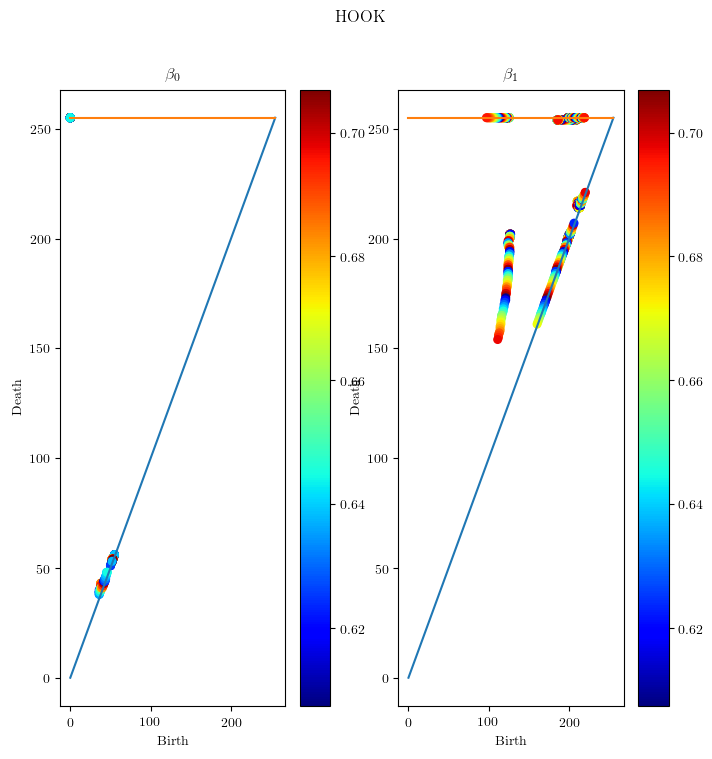
\includegraphics[width=\textwidth,height=.32\textheight]{MNG_hook_PDcolor}
\end{minipage}
\caption{ \label{fig:MNG_hookPDdiagram_likelywrong}
Persistence diagrams of the hook family of solutions
\reffig{fig:MNG_leftright_family}\,(d-f) for zeroth and first
Betti numbers. The coloring represent energy; the same qualitative coloring is
producing if you track the period of solutions or the spatial domain size. In other words
the continuity of the persistence diagrams cannot be described by system parameters.
}
\end{figure}

\MNGpost{2018-09-25}{
Including a figure of the persistence diagrams for the continuous family of solutions produced
by numerical continuation of the hook tile in domain size. The color coding represents the energy of the
solution; one can see that the coloring is not a nice continuous gradient therefore the family is not parameterized
by energy, nor is it parameterized by $T$ or $L$.

While I got the code running on light (it runs really quickly) I'm still
learning the details, specifically about the use of \emph{cubical complexes},
which I believe is just a way of approximating the infinitely dimensional
scalar field after it has been discretized, \ie, think of the scalar field as
a height map of rectangular prisms analogous to Riemann integration.

The horizontal lines of \reffig{fig:MNG_hookPDdiagram_likelywrong} represent ``infinity,'' \ie, there are features
that are born at a finite ``time'' (threshold value for level sets of cubes arranged in grid) and persist as the threshold
passes the maximum of the function.

The Betti number zero point at infinity makes sense and can be explained. For mathematical consistency whenever two
simply connected regions are merged the younger one dies; therefore the global minimum lives from the beginning until the end.

The Betti number one points along the infinity boundary make absolutely no sense to me and have convinced me that
I'm missing a small detail in the calculation thats giving me errant data. What these points imply is that there are holes
that persist past the maximum of the function, but at that point everything would be beneath the ``sea level'' leaving only
one Betti number zero region (as previously described). Yet despite this I get lots of points at infinite for Betti number one
persistence diagrams.

I believe that the code that produces correctly formatted text files is
correct. What I believe I needed to do (and therefore implemented this) is to
first map the values of the scalar field $u(x,t)$ to the 8\,bit integers $(z
\in (0,1, 2, \cdots, 255))$ as these numbers are sufficient (and necessary in
certain formats) to represent a grayscale image.

The transformation that I apply is to add the absolute value of the minimum value of the scalar field across the scalar field such that the global
minimum has a value of zero. Then, the scalar field is rescaled by dividing the values of the field by the sum of the old minimum plus old maximum,
which after the first transformation is the new global maximum value. This leaves us with a scalar field valued between zero and one; multiplying
by 255 and then casting the field from floats to integers leaves us with the correctly valued field.

The lexicographical ordering that is mentioned in my previous post is relatively straightforward, we just need a vector whose elements are ordered
such that they represent the values of the field going from left to right $x=0\rightarrow L$ starting at the bottom $t=0$ and ending at the top $t=T_p$.
This is easily accomplished by rearranging the array with built in functions in Python (numpy, scipy).

I thought that perhaps the errors were occurring because I had to manually make the field periodic as opposed to the normal representation where
the leftmost values $x=0$ do not equal the right most values $x=L$ but the connect is assumed; this is generally how discrete Fourier transforms
format the data. I tested this and the results made even less sense, so I'm going to attempt to see if I can get Brett Tregoning or Michael Schatz to
join us next week (this week is likely too short notice).
}

    \PCpost{2018-09-26}{
I do not think anyone of us can make sense of
\reffig{fig:MNG_hookPDdiagram_likelywrong} without seeing the corresponding
black-white diagram of the hook family
\reffig{fig:MNG_leftright_family}\,(d-f), in the spirit of video 1
\HREF{https://www.sciencedirect.com/science/article/pii/S0167278916000270}
{(click here)} from Schatz group's persistent homology paper\rf{KLTSPSM16}.

\MNGedit{Chose one constituent member of the family of solution to produce such an animation, located in
\texttt{figs} titled \texttt{animated\_PDhook0} which can be viewed via google chrome. }
    }
\begin{figure}[ht]
\begin{minipage}[height=.32\textheight]{.8\textwidth}
\centering \small{\texttt{(a)}}
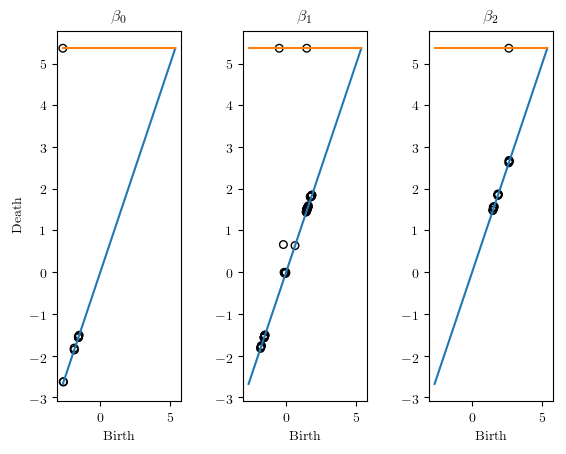
\includegraphics[width=\textwidth,height=.32\textheight]{MNG_threeD_family}
\end{minipage}
\caption{ \label{fig:MNG_threeD_family}
Persistence diagrams of the hook family of solutions for zeroth,first, and
second Betti numbers $\beta_0,\beta_1,\beta_2$. The persistent homology
calculation was performed by concatenating the family of solutions to form
a scalar field in three dimensions.
}
\end{figure}

\MNGpost{2018-09-27}{
{\bf [Numerical Continuation]}
Still working on the visualization for
persistent homology calculations, data management. The plan for tomorrow is
likely to numerical continue some solutions and then try to compute persistence
diagrams of the entire family and see if any useful information comes out.
}

\MNGpost{2018-09-27}{
{\bf [Persistent Homology]}
Spent a lot of time playing with persistent homology tools today.I went through a
variety of tests to gain intuition on persistence diagrams and ensure I
understand what they mean, and they are correct. I'm much more confident than I
was before today about what is actually going on with persistence diagrams,
especially the difference between components with different Betti numbers. I
searched for good examples of what the different numbers actually mean but I
found only the basic description of zero being simply connected regions, one
meaning ``one-dimensional holes'', and two being cavities.

I didn't really have an intuition for what constitutes a one dimensional hole,
but now I understand it is just a hole that you can draw a one dimensional curve
around, much like how a cavity is a hole that is enclosed by a two dimensional
surface. This explains the two points at infinity for tori, which are equivalent
to the direct product of two circles. Its these two circles that give rise to the
two infinitely persistent holes. The other, transient, holes on the persistence
diagram correspond to the torus not being completely filled in during the
thresholding process. An easy way to explain this is to think of the thresholding
process applied to the scalar field as coloring in the surface of the torus. Now
imagine this coloring process continues until almost all of the torus is filled
in except a small patch of the surface. This small patch would lead to a point on
the $\beta_1$ persistence diagram because you can draw a curve around it, and the
point at which the point dies is when this patch gets filled in.

These comments might seem obvious after the fact but I feel like there aren't
many people that attempt to explain it in an easy manner so I am going to do it
for myself. Many of the tests were sanity checks like, can I input the scalar
field information as real numbers?(yes). Does the data have to be periodic or is
periodicity assumed(has to be periodic)? Why are there births on the $\beta_1$
diagram when it appears as though nothing is happening? (It turns out that merely
sharing a vertex is sufficient to be connected in the ``cubical complex''
scheme).

I agree that \reffig{fig:MNG_hookPDdiagram_likelywrong} is terrible to look at,
especially because the color coding isn't labeled. After today's training I
thought of something that might be a good idea.
\reffig{fig:MNG_hookPDdiagram_likelywrong} is a superposition of an entire family
of solutions' persistence diagrams which is hard to analyze. Normally the scalar
fields that are being used to produce persistence diagrams are temporal snapshots
and so the natural means of visualizing this is a movie of persistence diagrams.
I don't know why this hasn't been done for the time series case, but instead of
attempting to parameterize the ``family'' of persistence diagrams, or make a
movie, why not just compute the persistent homology of the entire set of
snapshots at once; in other words my idea is to think of families of solutions as
a scalar field in three dimensions;two of which have periodic boundary
conditions.

This thought is what produced \reffig{fig:MNG_threeD_family}, which is the
persistence diagram computed for the entire family of numerically continued hook
solutions at different domain sizes at once. I am unsure as to whether the
different spatiotemporal domain sizes matters in this case, as I know (due to
Konstantin Mischaikow) that persistence diagrams are invariant under
homeomorphism, so if the rescaling transformation is a homeomorphism (which I
think is the case?) then it would not matter if the ``total'' transformation
comprised on individual two dimensional homeomorphisms is itself a homeomorphism.
One other problem is that in order to visualize the thresholding in this case
(The type of movie that makes the diagrams easy to understand as Predrag and I
both believe) it needs to be drawn in three dimensions which isn't easy and
likely not as enlightening. I believe this is an idea worth thinking through but
I am unsure if it is worth pursuing unless some interesting information comes out
of the consequent persistence diagrams.
\\

{\bf [Numerical Continuation and other codes]}
Still working on the initial condition generation for glueing together solutions
and symbolic dynamics, as well as numerical continuation, visualization for
persistent homology calculations, data management. The plan for tomorrow is
likely to numerical continue some solutions and then try to compute persistence
diagrams of the entire family and see if any useful information comes out.
\\

{\bf [Persistent homology calculations]}
The main takeaway seems to be numerical continuation of relatively large
solutions does not change the main features that much and so solutions
(subdomains, really) could possibly be identified by their persistence diagrams.

Although I put a decent amount of work into the three-dimensional family
versions of this code I think the single two-dimensional snap shot captures
all of the important information. The three dimensional representation just
shows that familes of solutions are continuous deformations of one another,
which we really already knew.

}

\begin{figure}[ht]
\begin{minipage}[height=.32\textheight]{1.0\textwidth}
\centering %\small{\texttt{(a)}}
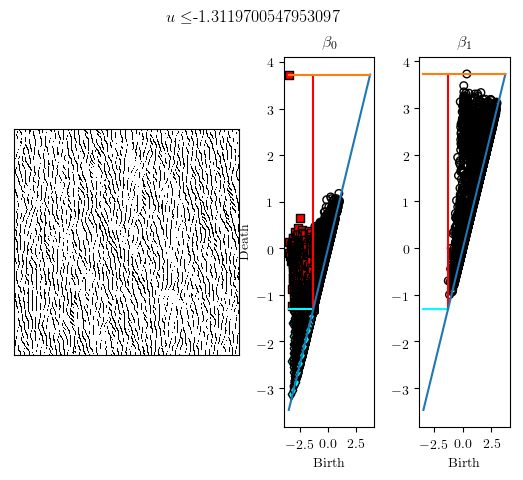
\includegraphics[width=\textwidth,height=.32\textheight]{MNGpers500b500}
\end{minipage}
\caption{ \label{fig:MNGpers500b500}
Persistence diagram for a large spatiotemporal trajectory (not periodic in time)
disaplying a particular thresholding value for the scalar field immediately
before and $\beta_1$ events are born occur (right figure).
}
\end{figure}

\MNGpost{2018-10-05}{
Trying to make up for lost time by working overtime during the week and
completely crashing on weekends. I'm hoping I can keep it up

\begin{description}
\item[Persistent Homology]
I'm only including one figure
I produced from a persistent homology calculation on segments of an ergodic trajectory,
$t \in [0,20]$,$t \in [0,40]$, etc. as the temporal extent of the time series was
increased the Betti number zero events seemingly get squashed into the bottom of the
persistence diagram and vice versa for the Betti number one events. In other words I guess
as one samples more and more of the attractor the persistence diagram asymptotically
approaches some regularized distribution. This could just be a red herring because
as one takes in more data the more regularized it will be. It's essentially the bottom third
of the range of values that the scalar field can take on is dominated by spots. Around the two
thirds point (as measured from the bottom of $[-u_{min},u_{max}]$) all of the black spots become
connected, which I find kind of surprising, due to the fact that it just seems to be at some arbitrary
value that long time series approach asymptotically. Likewise, for the one-dimensional holes, Betti number
one events, none exist until a certain threshold point. It could be meaningly less but perhaps after
accounting for noise one could derive a relation between persistence diagrams and solution, or characterize
the attractor as an asymptotic state in persistence diagram space. Something to ponder.

\end{description}
}

\begin{figure}
\begin{minipage}[height=.32\textheight]{.9\textwidth}
\centering \small{\texttt{(a)}}
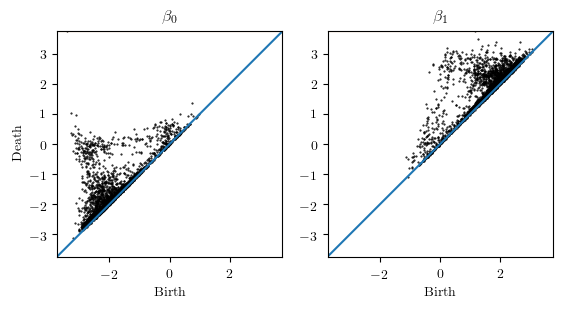
\includegraphics[width=\textwidth,height=.32\textheight]{MNG_PD_short}
\end{minipage}
\begin{minipage}[height=.32\textheight]{.9\textwidth}
\centering \small{\texttt{(b)}}
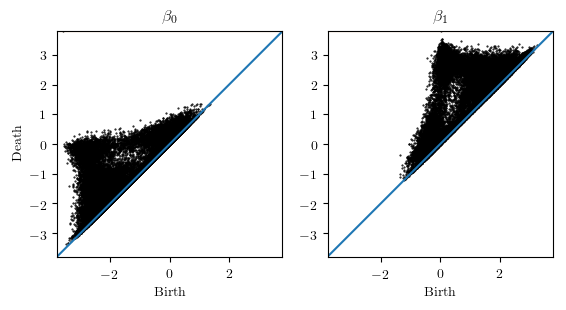
\includegraphics[width=\textwidth,height=.32\textheight]{MNG_PD}
\end{minipage}
\caption{ \label{fig:MNG_PD}
(a) Persistence diagram of ergodic segment with temporal extent $T=200$.
(b) Persistence diagram of ergodic segment with temporal extent $T=4800$, (includes (a) as
   the first $200$ time units)
}
\end{figure}

\begin{figure}
\begin{minipage}[height=.32\textheight]{.9\textwidth}
\centering
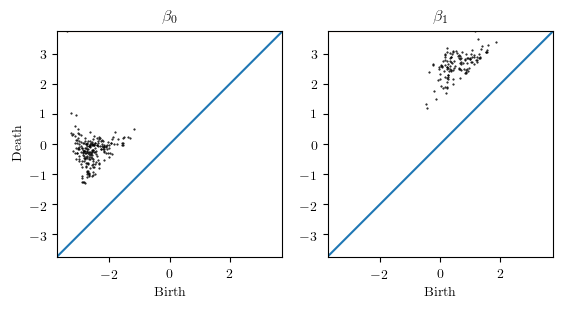
\includegraphics[width=\textwidth,height=.32\textheight]{MNG_PD_F_short}\\
\small{\texttt{(a)}}
\end{minipage}
\begin{minipage}[height=.32\textheight]{.9\textwidth}
\centering
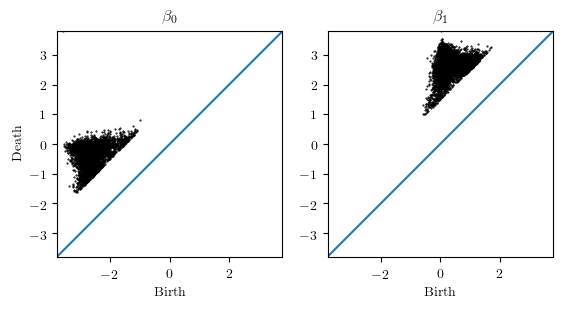
\includegraphics[width=\textwidth,height=.32\textheight]{MNG_PD_F}\\
\small{\texttt{(b)}}
\end{minipage}
\caption{ \label{fig:MNG_PD_F}
(a) Filtered persistence diagram (lifetime $\leq 1.5$ eliminated arbitrarily)
    of ergodic segment with temporal extent $T=200$
(b) Filtered persistence diagram
   of ergodic segment with temporal extent $T=4800$ ( includes (a) as
   the first $200$ time units)
}
\end{figure}

\begin{figure}
\begin{minipage}[height=.32\textheight]{1.0\textwidth}
\centering
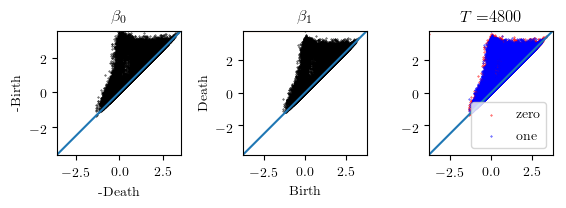
\includegraphics[width=\textwidth,height=.32\textheight]{MNG_PD_S}\\
\small{\texttt{(a)}}
\end{minipage}
\begin{minipage}[height=.32\textheight]{1.0\textwidth}
\centering
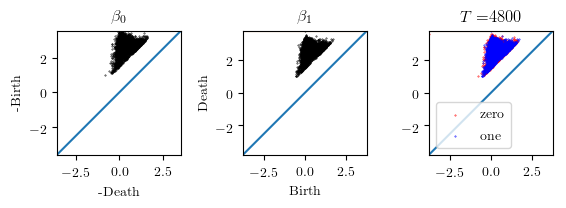
\includegraphics[width=\textwidth,height=.32\textheight]{MNG_PD_FS}\\
\small{\texttt{(b)}}
\end{minipage}
\caption{ \label{fig:MNG_PD_S}
Demonstrations of apparent reflection symmetry that relates reflections of the $\beta_0$ (simply connected regions persistence diagram) to
the $\beta_1$ (one-dimensional holes) persistence diagram.
(a) Persistence diagrams showing (left) reflected $\beta_0$, (middle) $\beta_1$ and (right) colored comparison.
(b) Filtered persistence diagrams showing (left) Reflected $\beta_0$, (middle) $\beta_1$ and (right) colored comparison.
Both (a) and (b) were computed for ergodic segment with temporal extent $T=4800$.
}
\end{figure}

\MNGpost{2018-10-10}{
\begin{description}
\item[Persistent homology of large ergodic segments]

In this post I will report on the recent results from applying the theory
of persistent homology to solutions of the Kuramoto-Sivashinsky equation.

Persistent homology calculations with small spatiotemporal solutions
has not yet provided anything fruitful, at least in my interpretation. Because
the solutions are defined on small domains there is no room
for very complex features and therefore the persistence diagrams have very few features.

I had the idea that perhaps the persistent homology of a long ergodic
segment might prove enlightening, as this is the opposite of the small spatiotemporal
area limit. I was unsure if the results were trivial so I reported them to Predrag
after the weekly plumbers meeting. Both of us found the results interesting
but couldn't really explain them.

(Side Note: I'm only going to provide the static persistence
diagrams for the ergodic trajectories because the spatiotemporal solution is too large to make
any sense out of the black and white spatiotemporal field being animated.)

An interesting observation is that there
seems to be two transitions. The first is where all thresholded regions become connected, the
second is a minimum value for loops to be born. This is slightly surprising to me. It makes
sense that there would be a maximum value after which everything is connected, but I would have expected
it to be much closer to the global maximum of the solution. More surprising is that no $\beta_1$ events
exist before a certain threshold; this is strange to me. It says that there is nowhere on the solution where
thresholded region make a ``loop'' until a certain minimum value. Perhaps this is not supposed to be surprising, as
the general behavior in time is of pairs of streaks, where successive minima are generally separated by maxima spatially.

Something that I found really interesting is that there appears to be a symmetry relation between the
Betti number zero and Betti number one diagrams. By reflecting the Betti zero $\beta_0$
events across the line $y=-x$ (technically $Death = -Birth$ using correct axis labels) maps the Betti zero
events to the approximate region of the persistence diagram that Betti one events populate. I don't know what this ``approximate symmetry'' means,
but if I had to bet I believe the most likely explanation is that it is a manifestation of reflection equivariance
of the \KSe\ and nothing more. Also, this is technically ignoring the infinite persistence points, I think this is
valid as these point are special and need to be considered separately.

The observations (without proof) that I believe are important are
\begin{itemize}
\item
    As $T \rightarrow \infty$ the region on the persistence diagrams where events
    exist becomes smaller. A mathy way of saying this is something along the
    lines of for a sequence of increasing $T_k$, the induced sequences of
    ``areas'' (as measured by, the convex hull of the set of points for instance)
    $A_k$ of the persistence diagrams follow the approximate rule $A_k+1
    \subseteq A_k$ and as $k \rightarrow \infty$, $A_k \rightarrow \bar{A}$,
    where $\bar{A}$ appears to be some statistically steady state. It could be
    that there is more going on under the multiple layers of data but the general
    idea that there is some asymptotic behavior I think is well merited. This
    convergence of the occupied regions in the persistence diagrams is
    demonstrated by computing multiple persistence diagrams for ergodic
    trajectory segments of varying temporal extents. In \reffig{fig:MNG_PD} (a)
    is the persistence diagram computed for the first $T=200$ time units of the
    ergodic segment and (b) is the first $T=4800$ units. This asymptotic behavior
    perhaps implies that some statistical information can be retrieved from
    persistence diagrams in the large $T$ limit.
\item
    The persistence diagrams looked like they had reflection symmetry over the
    line $y=-x$, and so I produced figures demonstrating this approximately. This
    is demonstrated for the unfiltered data and filtered data in of
    \reffig{fig:MNG_PD_S}\,(a) and (b) , respectively. The two regions overlap
    but it isn't an exact mapping as I had hoped. I'm still thinking through this
    but as I previously stated I believe that it is reflection equivariance
    shining through the data. I think I might test this by seeing what pops out
    when I perform the persistent homology computation on a trajectory in the
    antisymmetric subspace.
\item
    If events with lifetimes (death minus birth) less than a certain threshold
    are removed(i.e. require a minimum distance away from diagonal) the picture
    becomes more clear, especially the symmetry claim. This lifetime threshold
    was a guess to attempt to eliminate the least persistence information
    (near-diagonal eve\-nts). The filtering for two different time segments can
    be seen in \reffig{fig:MNG_PD_F}.
\end{itemize}

\end{description}

}

\MNGpost{2018-10-24}{
{\bf [Plumbers]}
We discussed the interesting information that seems to arise from performing
persistent homology calculations on large spatiotemporal domains (pieces of
ergodic trajectory). While currently in its early stages, we believe that the
asymptotic behavior captures statistical information about the inertial
manifolds; I'm going to produce a comparison between the large ergodic trajectory
and all \twots\ in the libraries I've formed to see if any interesting
comparisons can be made.
}


\PCpost{2018-10-29}{
Curious - is it possible that there is only one reference on the whole field of
persistent homology, the
Kram{\'a}r, Levanger, Tithof, Suri, Paul, Schatz and Mischaikow\rf{KLTSPSM16}
paper?
Or is that the only paper you have looked at?

The only other paper we have in \texttt{siminos.bib} is
Krishan, Kurtuldu, Schatz, Gameiro, Mischaikow and Madruga\rf{KKSGMM07}
{\em Homology and symmetry breaking in {Rayleigh-B{\'{e}}nard} convection:
{Experiments} and simulations}.
}

\PCpost{2019-04-05}{
Just to keep track of the activities in the field -
Jean-Philippe Lessard
(McGill University),
Jason D. Mireles James
(Florida Atlantic University)
and
Jan Bouwe van den Berg
(Vrije Universiteit Amsterdam)
gave an April 1, 2019 \HREF{http://www.crm.umontreal.ca/2019/Computer19/index_e.php}
{tutorial} on {\em A Computer-Assisted Constructive Approach to Nonlinear Dynamical Systems}.

This was followed by
a \HREF{http://www.crm.umontreal.ca/2019/Rigorous19/index_e.php} {workshop}
{\em Rigorous Computational Dynamics in Infinite Dimensions},
a \HREF{http://www.crm.umontreal.ca/2019/Framework19/index_e.php} {tutorial}
{\em A Topological-Combinatorial Framework for Dynamics},
and
a \HREF{http://www.crm.umontreal.ca/2019/Dynamique19/index_e.php} {workshop}
{\em Data Driven Dynamics: Algebraic Topology, Combinatorics and Analysis}.

Snippets:

``Some early successful applications of these methods for infinite dimensional
problems have been: [...] proving spatio-temporal behaviour in the
Kuramoto-Sivashinsky PDE;  [...]  and proving spontaneous periodic orbits in the
Navier-Stokes flow. ''

``Connecting orbits in ill-posed PDEs. Ill-posed PDEs (with no suitable initial
value problem) that come with a variational structure allow for the construction
of a Floer homology. Connecting orbits are essential ingredients of this
construction. If we can rigorously compute such connecting orbits, they yield
specific \emph{local} information, which when combined with generic global
analytic arguments, will lead to powerful forcing results.''

``explores the computational challenges of rigorously identifying and extracting
fundamental dynamical features such as equilibria, periodic orbits, connecting
orbits and invariant manifolds in infinite-dimensional dynamical systems.''

Mike Schatz is representing us this meeting:
\begin{enumerate}
  \item
    Dimension reduction. Data sets often have extremely high extrinsic
    dimension, but the information content is much lower dimensional. As an
    example, using Navier-Stokes as a model makes
    an infinite dimensional problem. Numerical simulations and
    experimentally collected data can easily involve million dimensional
    approximations. However, for many problems of interest the dimension of the
    attractor is on the order of 100 or less.
  \item
    \Statesp\ reconstruction from data. Typically only a subset of the relevant
    variables are observed. Therefore to capture the full dynamics requires some
    form of reconstruction of a model of \statesp.
  \item
    Information extraction. Typically the information of interest involves
    identification of dynamic structures or the possibility of prediction of
    dynamic behavior. Given that the input data is noisy and that steps 1 and 2
    involve processing the data, one needs robust techniques for extracting
    information.
\end{enumerate}

        }
\end{description}
%%%%%%%%%%%%%%%%%%%%%%%%%%%%%%%%%%%%%%%%%%%%%%%%%%%%%%%%%%%%%%%%%%%%%%%
\printbibliography[heading=subbibintoc,title={References}]
